\chapter{Evaluation}
\label{cha:evaluation}

\section{Datasets}
In this work, two datasets for segmentation and one for localization of surgical instruments are used for training and testing of the networks. 

\subsection{Endoscopic Vision Challenge 2017}
\label{sec:endovis17}

One segmentation dataset used in this work is part of the subchallenge Robotic Instrument Segmentation of the MICCAI Endoscopic Vision Challenge 2017. The subchallenge is divided into the tasks binary segmentation, part recognition, and type distinction of surgical instruments. 
Binary segmentation means that the instruments are distinguished from the background.~\cite{EndoVis17}
This challenge is abbreviated as \emph{EndoVis17-S}. 

\subsubsection{Robotic Training Data}
\label{sec:endovis17_training}
The eight training sets of EndoVis17-S consist of stereo camera images, each with a resolution of 1280$\times$1024~px (width$\times$height) acquired from a Da Vinci Xi robot~\cite{davindiXI2015morelli} during several different porcine procedures (see figure~\ref{img:original_endovis17_image}).
The ground truth for the camera images are hand annotated 1280$\times$1024~px greyscale images. It is provided for the part and type distinction task. These greyscale images are referred to as \emph{masks}.
For the part recognition task, each instrument part is encoded with different numerical values (see figure~\ref{img:mask_endovis17}).

\begin{figure}
\centering
\begin{subfigure}[t]{0.49\textwidth}
	\centering
	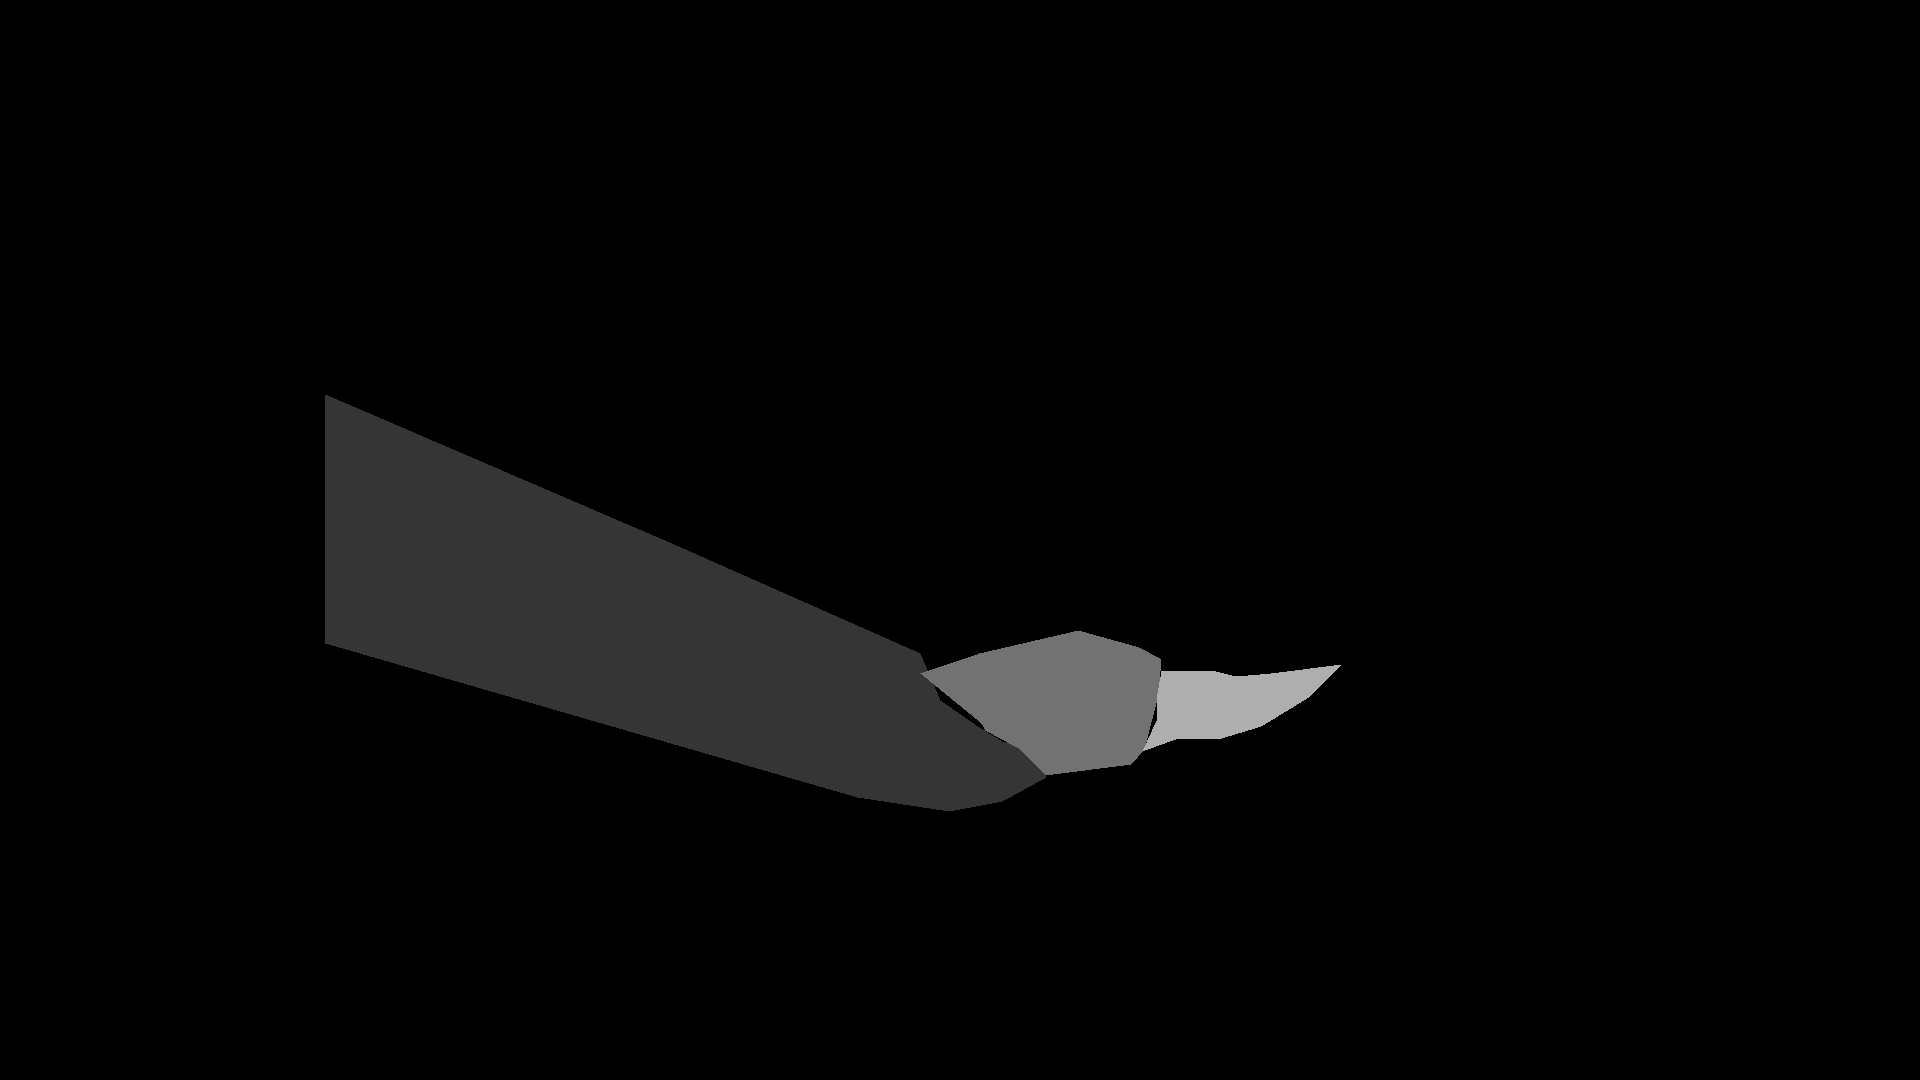
\includegraphics[width=.75\textwidth]{images/dataset/robotic17_segm/high_contrast_map_dataset1_maryland_frame009.png}
	\caption{Example ground truth with increased contrast and brightness for better visibility.}
	\label{img:mask_endovis17}
\end{subfigure}
\begin{subfigure}[t]{0.49\textwidth}
	\centering	
	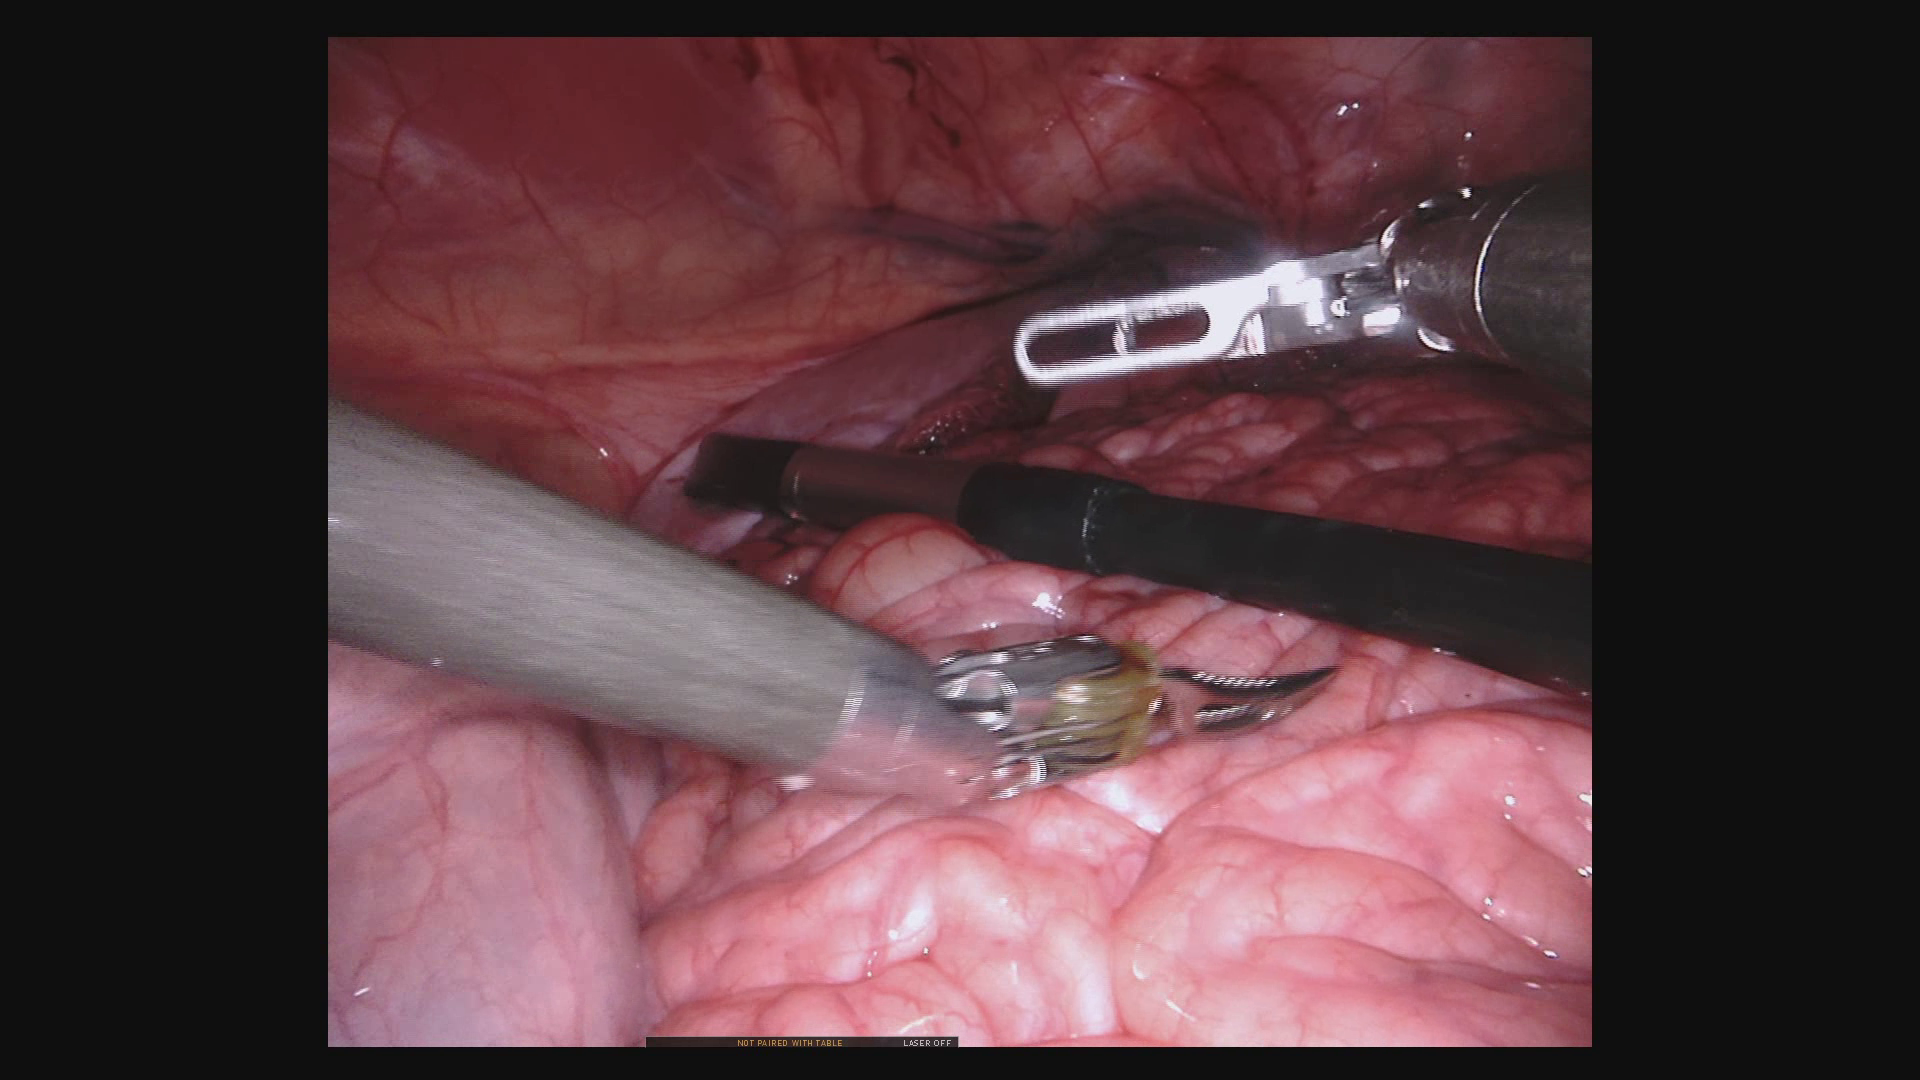
\includegraphics[width=.75\textwidth]{images/dataset/robotic17_segm/dataset1_frame009_3instruments.png}
	\caption{Example image with three instruments visible.}
	\label{img:original_endovis17_image}
\end{subfigure}
\caption[Example data EndoVis17-S]{Unmodified example image and corresponding ground truth for one instrument out of EndoVis17-S.}
\label{img:endovis17_orig_gt_and_image}
\end{figure}

For the instrument type distinction task, the ground truth for each instrument is provided separately: When more than one instrument is visible in the input image, each instrument has one ground truth image (see figure~\ref{img:endovis17_orig_gt_and_image}).

\subsubsection{Robotic Test Data}
The test data consists of eight datasets with 75 images each. They are acquired the same way as the training data. The test sequences were sampled immediately after each training sequence.
Additionally, there are two test sets with 300 images each. They contain different procedures than the eight datasets proposed for training.

\subsection{Endoscopic Vision Challenge 2015}
\label{sec:endovis15}
% decription that these are operation videos
% didn't use rigid -> describe only these ones & explain briefly.
Parts of the data used for this work are proposed in the subchallenge Instrument Segmentation and Tracking of the MICCAI Endoscopic Vision Challenge 2015~\cite{EndoVis15}. The subchallenge in general is abbreviated as \emph{EndoVis15}.

This subchallenge is separated into two dataset types: One \emph{rigid set} that contains only rigid surgical instruments and one \emph{robotic set} that contains only robotic surgical instruments.
The rigid set contains laparoscopic instruments during colorectal surgeries. It reflects typical challenges in endoscopic vision like occlusion, smoke and bleeding. 
In the robotic set, the instruments show typical poses and articulation in robotic surgery.  There is some occlusion, but no smoke and bleeding in any sequence.

This work only uses the robotic set. It is separated in a segmentation and a localization part.~\cite{EndoVis15}
The training and test inputs are the same, the ground truth is different for each part.
The segmentation part is abbreviated as \emph{EndoVis15-S}, the tracking part is abbreviated as \emph{EndoVis15-T}. 

\subsubsection{Robotic Training Data}
\label{sec:endovis15_robotic_train}
There are four robotic training sets. Each consists of a different 720$\times$576~px ex-vivo surgery video with 1100 frames per video and corresponding ground truth for each frame.
\emph{Ex-vivo} refers to procedures that are realized in an artificial environment outside a living organism.
The four surgeries are performed using the Da Vinci Surgical System~\cite{davinci2014watanabe}.

The first training set displays two instruments, the remaining three sets contain one instrument.

For EndoVis-S, the ground truth is provided as a greyscale video. For every frame, the (R,G,B) values of each pixel are labeled as background~(0,0,0), shaft~(160,160,160) or manipulator~(70,70,70) of the surgical instrument.

For EndoVis-T, the ground truth is provided as a text file where clasper angle, center point, and shaft axis of the instrument for every frame is listed (see figure~\ref{example_tracking}).

\begin{figure}
	\centering
	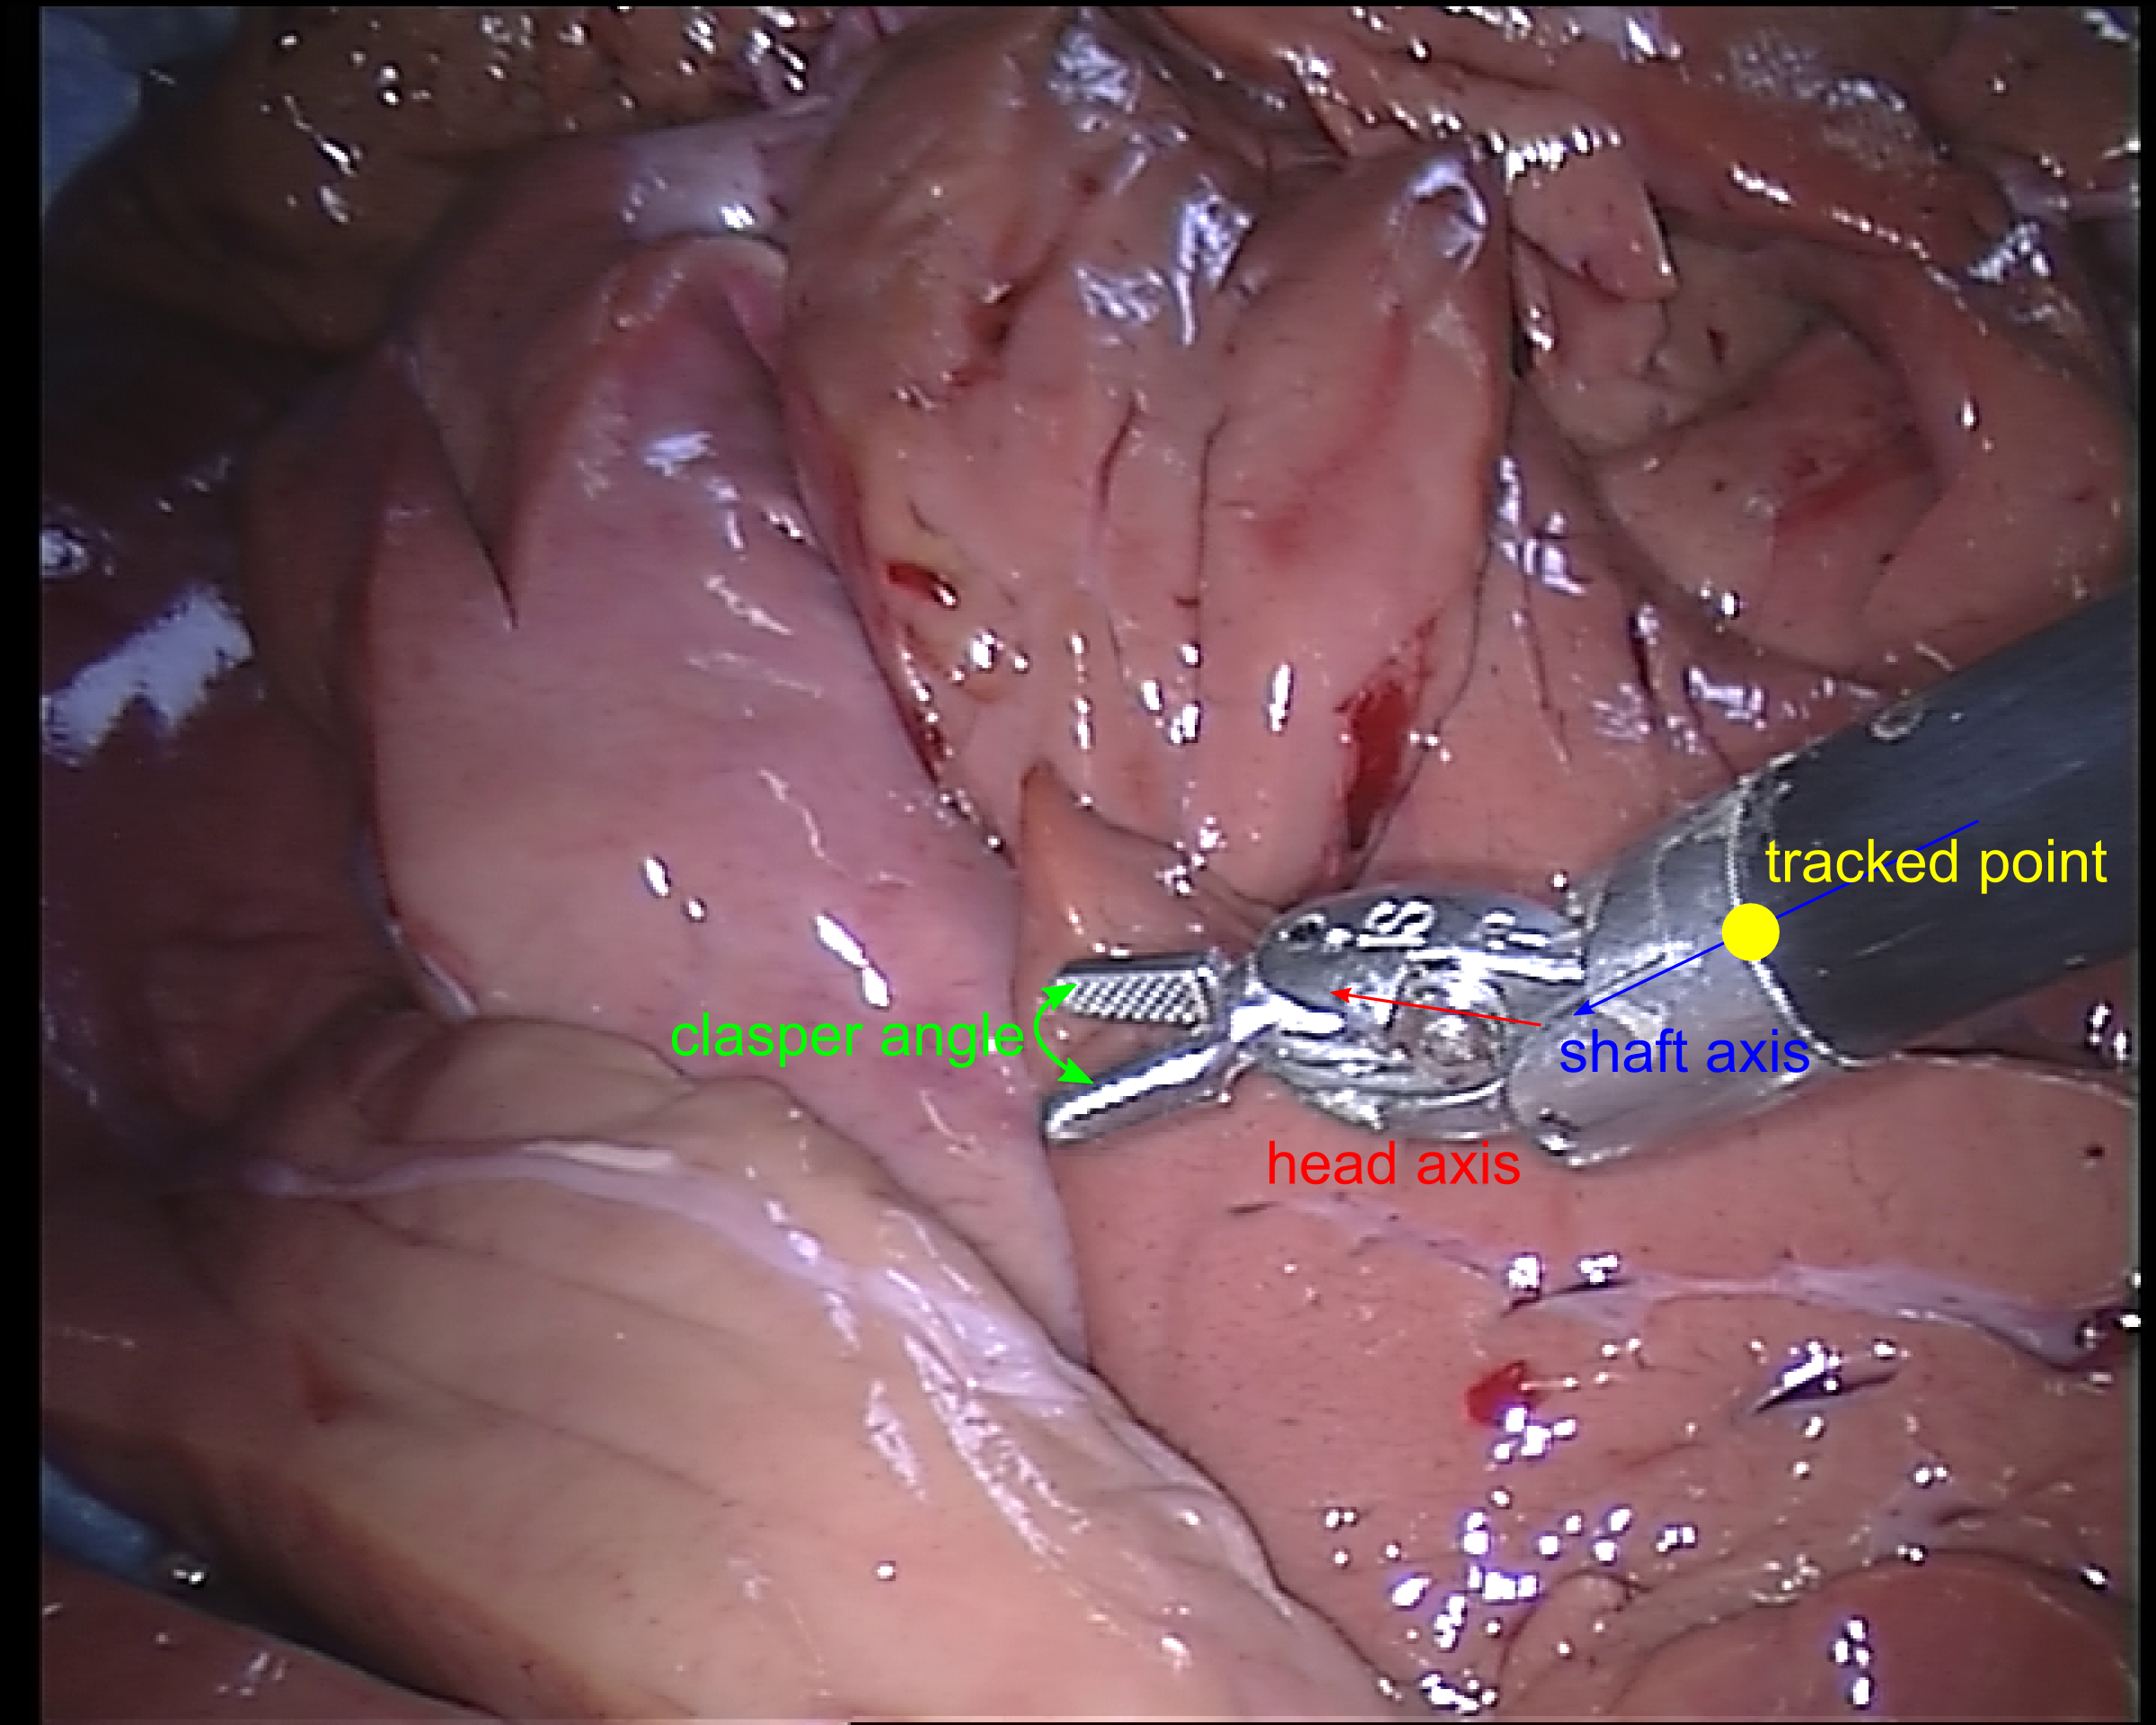
\includegraphics[width=.5\textwidth]{images/dataset/tracking_robotic15/guide_tracking.png}
	\caption[Example ground truth explanation EndoVis15-T]{Example image of EndoVis15-T provided by the challenge administrators to demonstrate the ground truth annotation for localization of the surgical instruments.}
	\label{example_tracking}
\end{figure}

\subsubsection{Robotic Test Data}
\label{sec:endovis15_robotic_test}
The robotic test data consist of 720$\times$576~px frames of additional video material for each of the four surgeries provided for training and two additional recorded surgeries with 1500 frames per video.

The ground truth for testing is provided the same way as for training.

The challenge guidelines specify two methods for testing the trained models.
The first method is a \emph{leave-one-surgery-out fashion (LOSO)}: For each of the four surgeries provided for training, one model is trained with the remaining three surgeries. The performance of the model is tested with the additional testing material for the one surgery that was not used for training. This is similar to $k$-fold cross validation (see also section~\ref{nn:testing}) with $k=4$.

The other testing method consists of training one model with the four surgeries provided for training and testing the performance with the two additional surgeries provided for testing.

\section{Data Preprocessing}
\label{sec:data_preprocessing}
To prepare the datasets for training and testing, several modifications have to be made to fit them for the network. 

\subsection{Endoscopic Vision Challenge 2017}
\label{sec:preprocess_endovis17}
The images of EndoVis17-S are surrounded by a black canvas (see figure~\ref{img:original_endovis17_image}). It is removed by cropping the images. This step is proposed in Shvets et al.~\cite{Shvets2018}
Without canvas, the images have a resolution of 1280$\times$1024~px.
The cropped images are downsampled to a resolution of 320$\times$265~px to decrease training time. 

\begin{figure}
\centering
\begin{subfigure}[t]{0.49\textwidth}
	\centering
	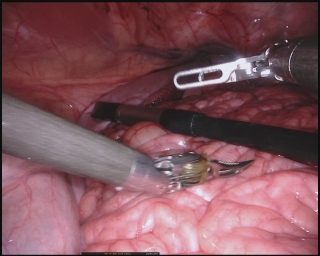
\includegraphics[width=.7\textwidth]{images/dataset/robotic17_segm/frame009_3instr_preprocessed.jpg}
	\caption{Preprocessed example image.}
	\label{img:preprocessed_train_img_segm17}
\end{subfigure}
\begin{subfigure}[t]{0.49\textwidth}
	\centering
	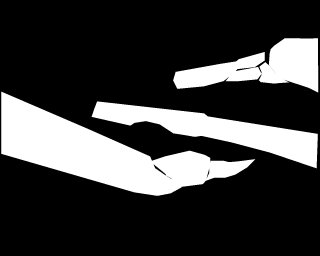
\includegraphics[width=.7\textwidth]{images/dataset/robotic17_segm/merged_dataset1_maryland_frame009.png}
	\caption{Preprocessed example mask: The three different instruments have the same colour.}
	\label{img:preprocessed_mask_segm17}
\end{subfigure}
\caption[Example data EndoVis17-S]{Example data provided for EndoVis17-S.}
\label{img:example}
\end{figure}

\begin{figure}
\centering
\begin{subfigure}[t]{0.49\textwidth}
	\centering
	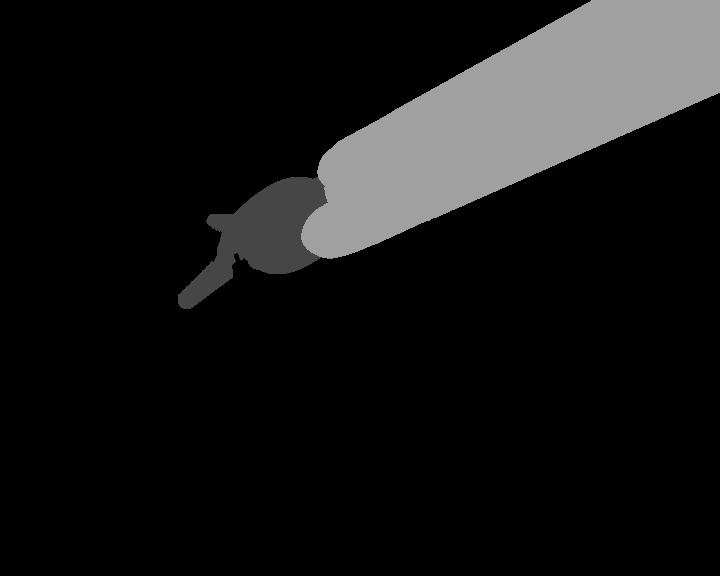
\includegraphics[width=.7\textwidth]{images/dataset/robotic15_segm/mask_original_dataset2_frame0.jpg}
	\caption{Original example mask with part annotations.}
	\label{img:orig_frame_endovis15}
\end{subfigure}
\begin{subfigure}[t]{0.49\textwidth}
	\centering
	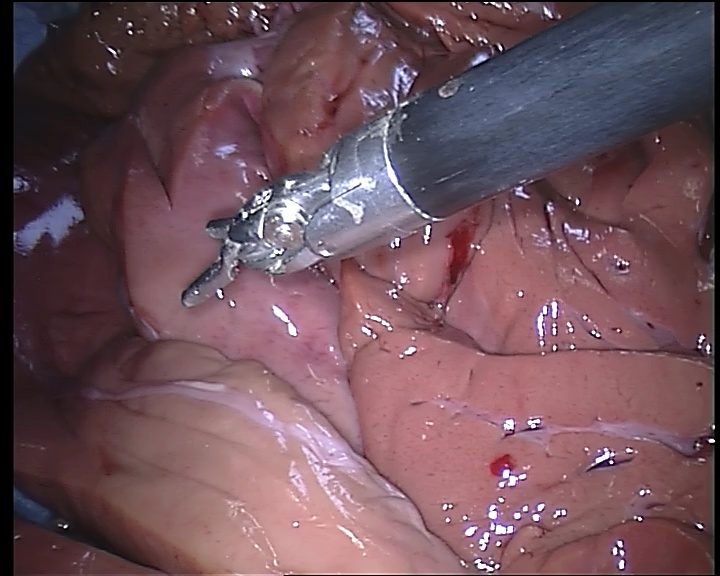
\includegraphics[width=.7\textwidth]{images/dataset/robotic15_segm/img_original_dataset2_frame0.jpg}
	\caption{Original example image.}
	\label{img:orig_mask_endovis15}
\end{subfigure}
\caption[Example data EndoVis15-S]{Unmodified example data provided for EndoVis15-S.}
\label{img:endovis15seg_orig_mask_image}
\end{figure}

Like the corresponding input images, the ground truth masks have a black canvas that has to be removed.
For the part recognition task of EndoVis-S (see figure~\ref{img:mask_endovis17}), the proposed masks have different greyscale values. As the networks in this work solve a binary segmentation problem, the greyscale masks are modified: The different greyscale values are reduced to two values~(R,G,B): Background (0,0,0) and instrument (255,255,255). For the type distinction task, every instrument has one single mask. When there is more than one instrument visible at the same time, their masks are merged into one image. 
After that, one binary mask contains the segmentation ground truth of all instruments shown in the corresponding input image. Like the corresponding input images, the masks are downsampled to a resolution of 320$\times$265~px~(see figure~\ref{img:preprocessed_mask_segm17}).

\subsection{Endoscopic Vision Challenge 2015}
\label{sec:prepocess_endovis15} 
The first preprocessing step for EndoVis15-S is extracting the images and masks out of the proposed videos.    
The resulting input images (see figure~\ref{img:orig_frame_endovis15}) and masks (see figure~\ref{img:orig_mask_endovis15}) have a resolution of 720$\times$576~px.
In order to give the EndoVis15-S data to the same network as the EndoVis17-S data, EndoVis15-S input images and corresponding masks are also downsampled to the resolution of 320$\times$265~px.

To prepare the masks for the binary segmentation task, the same adaptions as for \mbox{EndoVis17-S} are necessary:
The masks with greyscale values are converted into a binary image: Every pixel containing an instrument has the (R,G,B) value (255,255,255). The background pixels have the (R,G,B) value (0,0,0).
When two instruments are shown at the same time in one input image, the corresponding separated masks for each instrument are merged into one mask.

After the conversion to binary masks, erroneous white artefacts surrounding the instrument occur (see figure~\ref{img:white_artefacts_endovis15}).
When applying the operation opening (see Haralick et al.~\cite{opening1987haralick}), the white artefacts are reduced to such a low level that the masks can be used for training (see figure~\ref{img:mask_endovis15_after_morphology}).

\begin{figure}
\centering
\begin{subfigure}[t]{0.49\textwidth}
	\centering
	
\includegraphics[width=.65\textwidth]{images/dataset/robotic15_segm/white_artefacts_dataset1_frame21.jpg}
	\caption{After converting the ground truth images of EndoVis15-S to binary masks, they are surrounded by white artefacts.}
	\label{img:white_artefacts_endovis15}
\end{subfigure}
\begin{subfigure}[t]{0.49\textwidth}
	\centering
	
\includegraphics[width=.65\textwidth]{images/dataset/robotic15_segm/mask_after_morph_dataset1_frame21.jpg}
	\caption{After applying opening operation, the amount of white artefacts surrounding the instruments is reduced.}
	\label{img:mask_endovis15_after_morphology}
\end{subfigure}
\caption[Application opening operation on binary masks]{Binary masks out of EndoVis15-S before and after the application of opening operation~\cite{opening1987haralick}.}
\label{img:unprocessed_processed_masks_endovis15}
\end{figure}

% extracted only FIRST TWO vectors out of Pose.txt
The localization ground truth of the surgical videos is provided as a text file with instrument positions. These instrument positions are each converted into a heatmap, see section~\ref{sec:heatmaps}:
The standard deviation $\sigma$ (see equation~\ref{eq:gauss2D_function}) is set to 25. This way, the resulting Gaussian distribution around the center point of the instrument does not exceed the instrument itself, but is larger than a small point (see figure~\ref{img:superimposed_heatmaps}).

\begin{figure}
\centering
\begin{subfigure}[t]{0.49\textwidth}
	\centering
	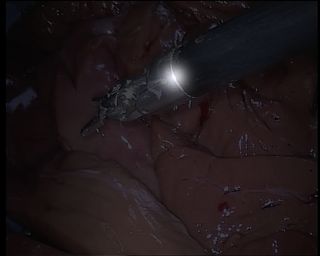
\includegraphics[width=0.7\textwidth]{images/dataset/robotic15_segm/img+heatmap_1instrument.png}
	\caption{Example image with superimposed corresponding heatmap.}
	\label{img:instr+heatmap}
\end{subfigure}	
\begin{subfigure}[t]{0.49\textwidth}
	\centering
	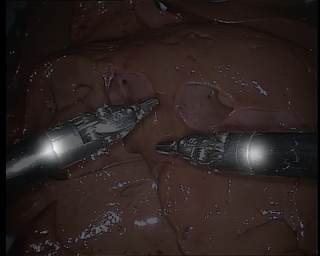
\includegraphics[width=0.7\textwidth]{images/dataset/robotic15_segm/image_frame001_superimposed_heatmap.png}
	\caption{Example image containing two instruments with superimposed corresponding heatmap.}
	\label{img:2instr+heatmap}
\end{subfigure}
\caption[Example image EndoVis15-T, corresponding heatmap]{Example images out of EndoVis15-T with corresponding heatmaps.}
\label{img:superimposed_heatmaps}
\end{figure}

Because the text file with the instrument center points is given for the original images with a size of 720$\times$576~px, the resulting heatmaps have the same size.
To fit them to the downsampled input images, the resolution of the heatmaps is reduced to 320$\times$265 pixels.

\section{Experiments}
After preprocessing the proposed datasets, TernausNet-11 (see section~\ref{sec:TernausNet_11}) and LocNet (see section~\ref{sec:tracking_net}) are trained and evaluated in different ways with EndoVis15-S, EndoVis17-S, and EndoVis15-T.

\subsection{Instrument Segmentation}
% (include example predicted masks)
Because TernausNet-11 is the basis network of LocNet, the segmentation task is evaluated on TernausNet-11 before using the evaluation results to improve the localization task.
The training and testing of the models trained with EndoVis15-S is performed according to the challenge guideline LOSO (see section~\ref{sec:endovis15_robotic_test}) of EndoVis15. All models were trained with batch-size 4.

% model #03: EndoVis15 only
The model \emph{TER-15S} is trained for 100 epochs with learning rate $\lambda=0.0001$ and 100 epochs more with $\lambda=0.00001$ on EndoVis15-S. 

% model #01: EndoVis15 + EndoVis17: 200 epochs 15, +100 epochs 17
% TER = TernausNet
% 15S = EndoVis15 segm set
% 200 = number of epochs
The model \emph{TER-15S-17S} is trained for 100 epochs with $\lambda=0.0001$ and 100 epochs with $\lambda=0.00001$ on EndoVis15-S.
Afterwards it is trained for 100 epochs with $\lambda=0.00001$ on EndoVis17-S. For the training on EndoVis17-S, the eight proposed training sets are divided in four subsets. Each of these subsets contains two training sets. These four subsets are used for training and testing the TER-15S-17S model with LOSO fashion on EndoVis15-S. 

For the results of both TernausNet-11 segmentation models see table~\ref{tab:training_results_seg}.

% Tabelle mit Ergebnissen für TRAININGSDATEN 4-fold (all correct now)
\begin{table}
\centering
 \begin{tabular}{l c c} 
 \hline\noalign{\smallskip}
 \multicolumn{3}{c}{\textbf{Segmentation Results TernausNet-11}} \\
  & TER-15S & TER-15S-17S \\ [0.5ex] 
 \hline
 epochs & 200 & 300 \\ [0.5ex]
% batch-size & 4 & 4 & 4 \\
% method & LOSO & LOSO & LOSO \\ 
 \hline \hline\noalign{\smallskip}
 precision & $92.77 \pm 6.35$ & $92.72 \pm 7.51$ \\
 b.acc. & $89.27 \pm 3.54$ & $88.26 \pm 7.07$ \\
 accuracy & $97.14 \pm 1.35$ & $96.94 \pm 2.04$ \\
 specificity & $99.32 \pm 0.62$ & $99.28 \pm 0.68$ \\
 recall & $79.22 \pm 6.78$ & $77.23 \pm 14$ \\
 IoU & $74.93 \pm 8.41$ & $73.39 \pm 14.29$ \\
 dice & $85.37 \pm 6.15$ & $83.73 \pm 11.32$ \\ [0.5ex]
 \hline
\end{tabular}
\caption[TernausNet-11 segmentation results]{Results of the different models for the segmentation of surgical instruments. Epochs denote the number of epochs for training in total. For evaluation metrics see section~\ref{sec:evaluation_metrics}. The evaluation results are given as mean value over all prediction results $\pm$ the standard deviation.}
\label{tab:training_results_seg}
\end{table}

%%% Discussion
%%% model TER-15S , model TER-15S-17S
The achieved results are comparable to other state-of-the-art approaches. 
TER-15S-17S was trained additionally with data from EndoVis17-S in order to test the impact of additional training data on the prediction performance of LocNet. 
The results for TER-15S and TER-15S-17S for testing on EndoVis15-S are in the same range, i.e. the additional data does not have an impact with high significance on the prediction capability of LocNet for EndoVis15-S. 
As the EndoVis17-S data are obtained during in-vivo procedures with seven different instruments, they differ from the EndoVis15-S data that were obtained in ex-vivo procedures with less different instrument types. Therefore, the information learned by the model out of EndoVis17-S does not have an improving effect on the prediction for EndoVis15-S.

\subsection{Concurrent Instrument Segmentation and Localization}
Each model is trained and evaluated according to one of the EndoVis15-T challenge guidelines: LOSO fashion (see section~\ref{sec:endovis15_robotic_test}), or training on all train sets and then testing on the test sets. 
For the specific training description of each model see table~\ref{tab:training_descr_locnet}.

\begin{table}
\centering
 \begin{tabular}{l c c c } 
 \hline\noalign{\smallskip}
 \multicolumn{4}{c}{\textbf{Training Conditions LocNet}} \\
	& epochs & val.method & $\gamma$  \\ [0.5ex]
 \hline \noalign{\smallskip}
 LOC-01 & 600 & LOSO & $1/2$ \\ 
 LOC-02 & 600 & LOSO & $2/3$ \\ 
 LOC-03 & 50 & LOSO & $1/2$ \\ 
 LOC-04 & 500 & T4 & $1/2$ \\
 LOC-05 & 100 & T4 & $1/2$ \\
 LOC-06 & 400 & LOSO & 1 \\
 LOC-07 & 100 & T4 & 1 \\ 
 LOC-08 & 500 & T4 & 1 \\ [0.5ex]
 \hline 
 \end{tabular}  
\caption[LocNet training conditions]{Validation method (val.method) specifies if the model was trained according to the LOSO fashion (LOSO), or trained completely on the four training sets and tested on the two test sets (T4). The impact of the segmentation and the localization loss on the model is adjusted by $\gamma$ (see section~\ref{sec:tracking_net}).}
\label{tab:training_descr_locnet}
\end{table}

For the segmentation results of all LocNet models see table~\ref{tab:segm_results_locnet}, for the localization results see table~\ref{tab:loc_results_datasets_LOSO} and table~\ref{tab:loc_results_datasets_T4}.

\begin{table}
\centering
 \begin{tabular}{l c c } 
 \hline\noalign{\smallskip}
 \multicolumn{3}{c}{\textbf{Segmentation Results LocNet}} \\
 & {b.acc.} & Dice \\ [0.5ex]
 \hline\noalign{\smallskip}
 LOC-01 & $88.45 \pm 1.8$ &$85.25 \pm 2.4$ \\ 
 LOC-02 & $\mathbf{90.65 \pm 1.7}$ & $\mathbf{87.8 \pm 2.3}$ \\ 
 LOC-03 & $89.75 \pm 4.1$  & $86.83 \pm 6.2$ \\ 
 LOC-04 & $87.45 \pm 2$ & $83.92 \pm 2.8$ \\
 LOC-05 & $89.45 \pm 2$ & $86.32 \pm 2.77$ \\ [0.5ex]
% LOC-06 & - & - \\
% LOC-07 & - & -\\ 
% LOC-08 & - & - \\ [0.5ex]
 \hline 
 \end{tabular}  
\caption[LocNet segmentation results]{Results of the different models for segmentation of surgical instruments. For evaluation metrics see section~\ref{sec:evaluation_metrics}. The evaluation results are given as mean value over all prediction results $\pm$ the standard deviation. As LOC-06, LOC-07, and LOC-08 are trained with loss factor $\gamma=1$, the segmentation results for these models are optimized for localization only.}
\label{tab:segm_results_locnet}
\end{table}

\begin{table}
\begin{adjustbox}{center=\textwidth}
\begin{tabular}{l c c c c c}
\hline\noalign{\smallskip}
\multicolumn{6}{c}{\textbf{Localization Results Datasets LOSO}} \\
 & Dataset1 left/right instr. & Dataset2 & Dataset3 & Dataset4 & mean dist.\\
\hline\noalign{\smallskip}
LOC-01 & $21.24 \pm 12.5 / 17 \pm 10.4$ & $13.45 \pm 5.9$ & $12.73 \pm 5.7$ & $14.22 \pm 23.5$ & $16.27 \pm 19.6$ \\
LOC-02 & $22.65 \pm 31.1 / 15.5 \pm 22.5$ & - & - & - & - \\
LOC-03 &  $\mathbf{17.58 \pm 12.1 / 15.15 \pm 9.4}$ & $\mathbf{11.36 \pm 6.4}$ & $\mathbf{10.83 \pm 6.3}$ & $\mathbf{12.05 \pm 8.9}$ & $\mathbf{13.85 \pm 10.0}$\\ 
LOC-06 &$372.24 \pm 91.7 / 299.62 \pm 251.1$ & $27.66 \pm 109.9$ & $20.47 \pm 82.13$ & $21.48 \pm 80.2$ & $152.5 \pm 207.9$ \\ [0.5ex] 
\end{tabular}
\end{adjustbox}
\caption[LocNet results leave-one-surgery-out]{Results for the different datasets for each LOSO LocNet model. All models were trained according to the LOSO fashion (LOSO).
Mean dist. is the mean distance over all datasets. Dataset1 is distinguished into left and right instrument (left/right instr.).
The evaluation results are given as mean value over all prediction results $\pm$ the standard deviation. The distance between ground truth location and predicted location of the instrument is given in pixels.}
\label{tab:loc_results_datasets_LOSO}
\end{table}


\begin{table}
\begin{tabular}{l c c c}
\hline\noalign{\smallskip}
\multicolumn{4}{c}{\textbf{Localization Results Datasets T4}} \\
 & Dataset5 left/right instr.& Dataset6 left/right instr.& mean dist.\\
 \hline\noalign{\smallskip}
LOC-04 &  $89.80 \pm 101.1 / \mathbf{117.91 \pm 69.0}$ & $\mathbf{88.17 \pm 91.2} / \mathbf{120.02 \pm 68.2}$ & $\mathbf{106.4 \pm 80.4}$\\
LOC-05 & $\mathbf{69.59 \pm 51.6} / 118.15 \pm 73.2$ & $100.15 \pm 118.8 / 120.32 \pm 70.0$ & $111.7 \pm 94.5$\\ 
LOC-07 &  $114.13 \pm 136.8 / 121.51 \pm 78.8$ & $215.36 \pm 225 / 122.23 \pm 73.5$ & $162.04 \pm 163.9$ \\ 
LOC-08 & $121.5 \pm 146.5 / 122.43 \pm 80.9$ & $231.56 \pm 229.3 / 123.5 \pm 77.5$ & $169.7 \pm 169.7$ \\ [0.5ex]
\end{tabular}
\caption[LocNet results tests EndoVis15-T]{Results for the different datasets for each T4 LocNet model. T4 denotes that the models were trained completely on the four training sets and tested on the two test sets.
Each dataset is distinguished into left and right instrument (left/right instr.).
Mean dist. is the mean distance over all datasets. The evaluation results are given as mean value over all prediction results $\pm$ the standard deviation. The distance between ground truth location and predicted location of the instrument is given in pixels.}
\label{tab:loc_results_datasets_T4}
\end{table}

As the instrument positions are extracted from the heatmaps with k-means clustering and k is set to the number of instruments expected to be seen in the input frame, when the number of instruments actually seen in the input frame differs, the localization results are distorted. 
Another problem is that when the center point of an instrument is disappearing for a certain period of frames, but not the complete instrument, the prediction of the model will still contain higher pixel values, yielding a false-positive localization result for the partly visible instrument. This is because the model predicts a Gaussian distribution surrounding the center point, so even when the center point is not visible, the spread of the Gaussian is contained in the prediction (see figure~\ref{img:nearly_disappeared_instr}). 
In this case, comparing the estimated instrument location to the ground truth leads to unreasonably bad results, since the ground truth location for a center point not shown in the image is $(-1, -1)$ and not the actual instrument location. For this reason, the frames where the center point of the instruments is missing according to the ground truth annotation are excluded from evaluation.

To solve the problems in general, further postprocessing steps could be taken:
By checking the distance between the cluster center points, the case when two expected heatmaps are collapsed into one could be recognized, which would indicate that only one of the two instruments is visible.
%could be setting the distance between the predicted center points as a threshold to annotate the center point of one instrument as invisible to solve the k-means clustering problem.
Setting a threshold for the amount of higher pixel values found in the predicted heatmap to recognize frames where the center point is probably missing, could solve the general disappearing instrument problem.

\section{Discussion}
%As the values of the segmentation evaluation are in the range of current state-of-the-art results, 
The models trained according to LOSO fashion vary in number of epochs and the loss factor~$\gamma$.
LOC-01 and LOC-03 only differ in the number of epochs. The evaluation results are in the same range, but LOC-03 trained with 50 epochs outperforms LOC-01 which is trained with 600 epochs. 
The resulting heatmaps for LOC-01 look different from LOC-03 for Dataset1, the spread of the Gaussian distribution contains a higher variance for LOC-01 (see figure~\ref{img:pred_heatmap_high_variance}).

\begin{figure}
\centering
\begin{subfigure}[t]{0.49\textwidth}
\centering

\includegraphics[width=.7\textwidth]{images/predictions/model1/nearly_vanished_instr/frame308_nearly_disappeared.jpg}
\caption{Example heatmap prediction where the instrument center point is not visible in the input image.}
\label{img:nearly_disappeared_instr}
\end{subfigure}
\begin{subfigure}[t]{0.49\textwidth}
\centering

\includegraphics[width=.7\textwidth]{images/predictions/model3/Dataset1-high_variance/frame037_heatmap_high_variance.jpg}
\caption{Example heatmap prediction with high variance.}
\label{img:pred_heatmap_high_variance}
\end{subfigure}
\caption[Example heatmap prediction high variance, example heatmap prediction disappearing center point]{Example of two heatmap predictions: (a) Heatmap prediction where the instrument center point is disappearing. Notably, the prediction does only contain a low range of pixel values because of the missing center point. (b) Heatmap prediction of LOC-01 with high variance.}
\label{img:high+low_variance_heatmaps}
\end{figure}

This indicates that LOC-03 does not find the center point with high certainty, but the resulting location values are still slightly better than for LOC-01. This could be because the distribution of the Gaussians around the center points are still separated sufficiently, so it is possible to determine the center points with k-means clustering with a high accuracy. As LOC-03 is trained with less epochs than LOC-01, this could indicate that LOC-03 generalizes better and LOC-01 is overfitted on the training data.
LOC-02 differs from LOC-01 only in the size of $\gamma$: The impact of the localization loss is $2/3$, the impact of the segmentation loss is $1/3$.
The resulting values for Dataset1 are slightly worse than for LOC-01 and LOC-03. The resulting heatmaps contain Gaussian distributions with high variance.
For LOC-06, $\gamma$ is set to 1, therefore the impact of the segmentation loss is set to 0. It is trained 350 epochs more than LOC-02. For the LOSO method, this model achieves the lowest results, especially for Dataset1. As Dataset1 is the only dataset where two instruments are shown, and therefore LOC-06 tested on this dataset has not seen more than one instrument during training, it is possible that the missing segmentation information makes it more difficult for the network to predict a previously unseen number of instruments.

The models trained according to T4 fashion vary in the number of epochs and the loss factor~$\gamma$.
LOC-04 differs from LOC-05 in the number of epochs, it is trained 400 epochs more than LOC-05. $\gamma$ is set to four for both models, therefore the segmentation and localization loss have the same impact. The results for both models are in the same rage.
The models LOC-07 and LOC-08 are trained with $\gamma=1$, the impact of the segmentation is set to 0. LOC-08 is trained with 400 epochs more than LOC-07. The results for LOC-08 are lower than for the other proposed T4 models.
The evaluation results for the T4 models differ from the results for the LOSO models with an inaccuracy of more than 70~pixels. Notably, the ground truth annotations for the test datasets Dataset5 and Dataset6 seem to be inaccurate: This is stated by the challenge administrators~\cite{Laina2017}, an example can be seen in figure~\ref{img:wrong_test_gt_exampe+pred}. % Dataset5 -> 1st predicted frame LOC-08 / LOC-07, gt annotation for this frame --> merge in gimp

\begin{figure}
\centering
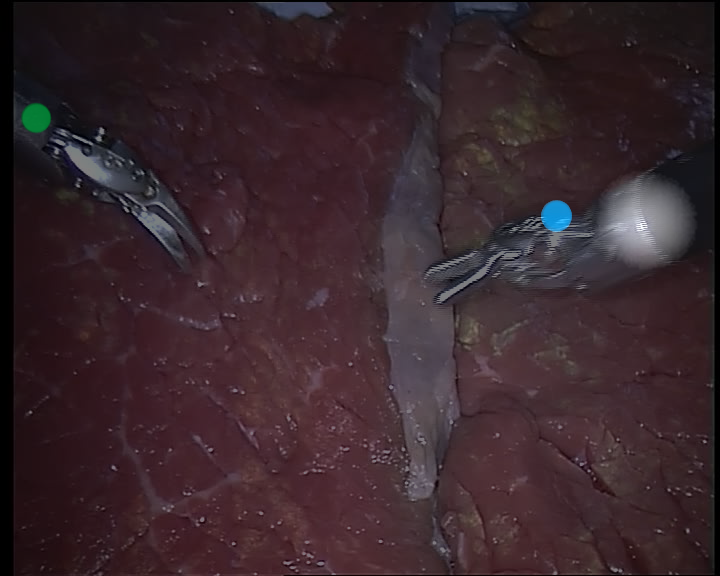
\includegraphics[width=.5\textwidth]{images/predictions/model7/frame001_superimposed_perd_and_gt.png}
\caption[Example image ground truth annotation]{Example input image with superimposed predicted preprocessed heatmap by LOC-07. The given ground truth for the left instrument is denoted in green, for the right instrument in blue. Notably, the center point of the left instrument is not visible, and the center point of the right instrument is actually positioned right from the ground truth annotation.}
\label{img:wrong_test_gt_exampe+pred}
\end{figure}

In summary, the best LOSO model is LOC-03 and the best T4 model is LOC-04. This indicates that setting $\gamma$ to 0.5 yields models with good prediction results.

\subsection{Comparison to State of the Art Methods} 
%The performance of the proposed neural network is compared to other methods using the same dataset and the same evaluation metrics.
The values for segmentation evaluation are in the same range as the current state-of-the-art results, except for the models trained with loss factor $\gamma=1$.

For training method LOSO, the evaluation results for localization outperform the state-of-the-art methods with the models LOC-01 and LOC-03. 
For training method T4, the evaluation results are lower or similar to the state-of-the-art methods.

\subsection{Future Work}
%The localization information obtained by the methods proposed in this work can be used for tracking models. The localization output of the instruments given over time can be used for tracking of surgical instruments during surgery. 
%When the input to the network is occluded by smoke or blood resulting of the surgery procedure, the location of the instrument could still be detected by usind Kalman filtering.
Besides taking further postprocessing steps to improve results, the proposed method could be combined with a temporal tracking algorithm. In this case, the estimated instrument locations could serve as input to trackers such as Kalman filter or Particle filter~\cite{kalman_filter1992brown}. Temporal tracking would be especially helpful to deal with occlusions and to associate each heatmap with either the left or the right instrument, even when instruments cross.
